\pstart%
Impetus\protect\index{Sachverzeichnis}{impetus} acquisitos in fine esse eosdem,
\edtext{sive in perpendiculari,}{\lemma{sive}\Bfootnote{\textit{(1)}\ recta \textit{(2)}\ in perpendiculari \textit{L}}}
sive in inclinata descendat grave,\protect\index{Sachverzeichnis}{grave}
facile ex his demonstratum est,
\edtext{nam ut}{\lemma{nam}\Bfootnote{\textit{(1)}\ et \textit{(2)}\ ut \textit{L}}}
major linea decurritur, et
\edtext{impetus\protect\index{Sachverzeichnis}{impetus} primus, et proinde singuli acquisiti sunt}{\lemma{impetus}\Bfootnote{%
\textit{(1)}\ singuli sun %
\textit{(2)}\ primus [...] sunt \textit{L}}}
minores in ea ratione qua linea est major,
cum \edtext{ergo impetus obliquus ultimus sit ad obliquum primum ut linea descensus est ad}{\lemma{ergo}\Bfootnote{%
\textit{(1)}\ quanti %
\textit{(2)}\ impetus %
\textit{(a)}\ et multiplicentur %
\textit{(b)}\ ultimus %
\textit{(aa)}\ sit %
\textit{(bb)}\ exprimi possit linea %
\textit{(cc)}\ sit ad primum ut linea descensus ad %
\textit{(cc)}\ obliquus [...] est ad \textit{L}}}
primum suum punctum,
et quanto linea inclinata major est linea tendentiae,\protect\index{Sachverzeichnis}{linea tendentiae}
\edtext{tanto impetus}{\lemma{tanto}\Bfootnote{\textit{(1)}\ linea \textit{(2)}\ impetus \textit{L}}}
sit minor, summa impetuum\protect\index{Sachverzeichnis}{impetus} erit aequalis.
Impetum\protect\index{Sachverzeichnis}{impetus} autem inclinatum esse ad perpendicularem,
ut perpendicularis ad inclinatam ad eandem basin demissam
\edtext{alibi}{\lemma{alibi}\Cfootnote{Stelle nicht nachgewiesen.}}
demonstratum est. 
\edtext{Unde demonstratur}{\lemma{Unde}\Bfootnote{\textbar\ invertendo facile \textit{gestr.} \textbar\ demonstratur \textit{L}}}
tempora
\edtext{descensus perpendicularis ad descensum inclinatum, esse ut perpendicularis}{\lemma{descensus}\Bfootnote{%
\textit{(1)}\ quoque esse ut linea %
\textit{(2)}\ perpendicularis ad [...] ut perpendicularis \textit{L}}}
est ad inclinatam.
Nam si aequale esset, essent impetus\protect\index{Sachverzeichnis}{impetus} seu vires acquisitae in ratione spatiorum,
ergo \edtext{cum vires sint}{\lemma{cum}\Bfootnote{\textit{(1)}\ impetus \textit{(2)}\ vires sint \textit{L}}}
aequales, erunt tempora in ratione spatiorum.
\pend
\newpage
\count\Afootins=1200
\count\Bfootins=1000
\count\Cfootins=1200
\pstart
\centering
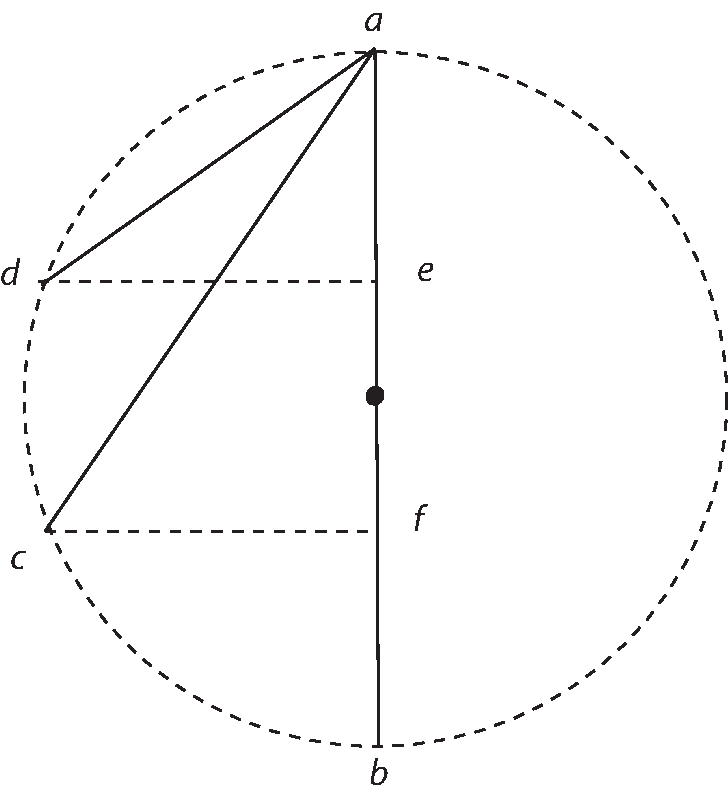
\includegraphics[width=0.44\textwidth]{images/lh03705_129r-d.pdf}\\
 \noindent \centering [\textit{Fig. 4}] 
\pend
\vspace{1.2em}
\pstart
\noindent%
\lbrack%
\textit{Nachfolgend klein gedruckter Text gestrichen:}\rbrack 
\pend
\vspace{0.4em}
\pstart%
\noindent%
\footnotesize%
Hinc \setline{2}porro sequitur,
\edtext{si grave}{\lemma{si}\Bfootnote{%
\textit{(1)}\ vi \textit{(2)}\ tem \textit{(3)}\ duo sint plana e \textit{(4)}\ corpus \textit{(5)}\ grave \textit{L}}}
\edtext{labi}{\lemma{labi}\Bfootnote{\textit{erg. L}}}
intelligatur ex eodem puncto libere nunc in plano inclinato,\protect\index{Sachverzeichnis}{planum inclinatum}
lineas aequalibus temporibus percursas fore inaequales, et maximam quidem fore perpendicularem.
Sed ut determinetur eorum ratio sic
\edtext{procedemus. Sunto}{\lemma{procedemus}\Bfootnote{\textit{(1)}\ , esto \textit{(2)}\ . Sunto \textit{L}}}
lineae descensus diversarum inclinationum, eodem tempore percursae
\edtext{\textit{ab.} \textit{ac.} \textit{ad.} lineae \textit{ad} et \textit{ac} absolvuntur eodem tempore. Impetus in prima}%
{\lemma{\textit{ab.} \textit{ac.} \textit{ad.}}\Bfootnote{%
\textit{(1)}\ Impetus in linea %
\textit{(2)}\ Ergo si duae descensiones comparentur inter se, impetus sunt ut lineae reciproces, %
at tres impetus inter se terminis fixis comparari non possunt. %
Comparatis ergo duobus insistamus: %
\textit{(3)}\ lineae [...] in prima \textit{L}}}
est ut $ac$, in secunda ut $af$, in tertia
\edtext{ut $ab$. Nam}{\lemma{ut $ab$.}\Bfootnote{\textit{(1)}\ Cum enim \textit{(2)} Nam \textit{L}}}
\edtext{impetus\protect\index{Sachverzeichnis}{impetus} quaesitus}{\lemma{impetus}\Bfootnote{\textit{(1)}\ initiales sin \textit{(2)}\ quaesitus \textit{L}}}
post percursam \textit{ad}
\edtext{vel \textit{ac} est aequalis}{\lemma{vel $ac$}\Bfootnote{\textit{(1)}\ fit ae \textit{(2)}\ est aequalis \textit{L}}}
impetui quaesito post percursam \textit{ae} vel \textit{af}.
\pend
\pstart 
\footnotesize
Idem ergo est
\edtext{impetus\protect\index{Sachverzeichnis}{impetus}}{\lemma{impetus}\Bfootnote{\textit{erg. L}}}
ac tria aequalibus temporibus percurrissent
\edtext{unum lineam}{\lemma{unum}\Bfootnote{\textit{(1)}\ spatium \textit{(2)}\ lineam \textit{L}}}
\textit{ae.} alterum \textit{af.} tertium \textit{ab.}
quo casu impetus\protect\index{Sachverzeichnis}{impetus} erunt ut lineae.
Iam cum impetus\protect\index{Sachverzeichnis}{impetus}
\edtext{quaesiti}{\lemma{quaesiti}\Bfootnote{\textit{erg. L}}}
sint ut lineae
\edtext{\textit{ae.} \textit{af.} \textit{ab}, et impetus primi sint ut lineae}%
{\lemma{\textit{ae.} \textit{af.} \textit{ab},}\Bfootnote{%
\textit{(1)}\ erunt lineae %
\textit{(2)}\ et lineae diversarum inclinationum, eodem tempore percursae eodemque impetu percursae, sint ut lineae %
\textit{(3)}\ et lineae diverso tempore %
\textit{(4)}\ et impetus primi sint ut lineae %
\textbar\ lineae diversarum inclinationum eadem celeritate eodem tempore, eodemque impetu percur \textit{gestr.} \textbar\ \textit{L}}}
[\textit{der Satz bricht ab.}]
\pend
\newpage
\pstart Hactenus ratiocinati sumus, supposito mobile in quolibet spatii puncto, impetum\protect\index{Sachverzeichnis}{impetus} accipere novum, priori aequalem, idque sive descensio sit in plano perpendiculari, sive in inclinato\protect\index{Sachverzeichnis}{planum inclinatum}, semper
[129~v\textsuperscript{o}]
enim res eodem redit.
\pend
\count\Bfootins=1200
\pstart%
Et necesse est descendentia per rectum inclinatumve in fine impetum\protect\index{Sachverzeichnis}{impetus} acquirere eundem.
\pend 
\pstart%
At sequuntur aliae conclusiones differentes a Galilaeanis, nimirum \edtext{Galilaeus,\protect\index{Namensregister}{\textso{Galilei}, (Galilaeus, Galileus), Galileo 1564-1642} assumens in quolibet momento impetum\protect\index{Sachverzeichnis}{impetus} accipi novum, ostendit spatia a  principio lationis assumta, aequalibus temporibus percursa fore ut quadrata temporum.}{\lemma{Galilaeus [...] temporum}\Cfootnote{\cite{00050}G. \textsc{Galilei}, \textit{Discorsi}, Leiden 1638 S. 171f. (\cite{00048}\textit{GO} VIII, S. 209f.).% (Discorsi, III, De motu naturaliter accelerato, Theorema II)
}}
Sint enim tempora \textit{ac}, \textit{ad}, erunt spatia  percursa\protect\index{Sachverzeichnis}{spatium percursum} ut Triangula \textit{aic}, \textit{akd}.
\pend 
\pstart
En ergo dubitationem insignem, quae certa demonstratione removenda
\edtext{est.}{\lemma{}\Afootnote{Fabri,\protect\index{Namensregister}{\textso{Fabri}, Honoré 1607-1688)}
ut in \textso{methodo scientiarum}\textsuperscript{[a]} ait,
credidit impetus\protect\index{Sachverzeichnis}{impetus} crescere,
ut numeros naturales ab unitate deinceps.\vspace*{2mm}\\%
\footnotesize%
\textsuperscript{[a]} \textso{scientiarum} \textit{erg. L}
% PR: Rein provisorisch !!!
\vspace*{1em}}}
Demonstrandum ergo spatium sumi non posse pro mensura, \edtext{et ineluctabilis}{\lemma{et}\Bfootnote{\textit{(1)}\ verissima de \textit{(2)}\ ineluctabilis \textit{L}}} ratio est, quia, si  spatium sumitur pro mensura, alius orietur \edtext{calculus, in eodem loco, tempore, motu mobile,}{\lemma{calculus,}\Bfootnote{%
\textit{(1)}\ si idem gra %
\textit{(2)}\ in eodem %
\textit{(a)}\ numero %
\textit{(b)}\ loco, %
\textit{(aa)}\ motu %
\textit{(bb)}\ tempore, motu mobile, \textit{L}}} prout progredi aut quiescere \edtext{supponitur[;] quod est absurdum.}{\lemma{}\Afootnote{Puto demonstrari rationibus, et argumentis firmari posse, corpus lapsum attollere posse tot corpora similia, quot altitudo ejus capit in altitudinem paulo minorem, qui est ipsius labentis. Idque elegantissimae observationis arbitror. An forte id falsum et ea huius rei aestimatio quae penduli. Ideo pendulum\protect\index{Sachverzeichnis}{pendulum} examinandum in diversis liquoribus.}} Item quod celerius movetur plus lucrabitur  proportionaliter, quam quod tardius movetur, quia plus loci percurrit, ita autem locus mensura erit. Eorum tempore pro mensura supposito, demonstrari puto potest, eundem impetum\protect\index{Sachverzeichnis}{impetus} acquirere gravia\protect\index{Sachverzeichnis}{grave} in plano inclinato\protect\index{Sachverzeichnis}{planum inclinatum} aut perpendiculari descendentia; descendunt enim in temporibus quae sunt ut \edtext{spatia, ergo}{\lemma{spatia,}\Bfootnote{\textbar\ reciproce \textit{erg. u. gestr.} \textbar\ ergo \textit{L}}} si in tempora ducantur, idem est, quasi ducantur in spatia, nam  impetus\protect\index{Sachverzeichnis}{impetus} minor in quadam ratione, ducitur in tempus majus eadem ratione. Ergo producta aequalia.
\pend 
\newpage
\pstart Impetus acquisitus per motum est ad impetum\protect\index{Sachverzeichnis}{impetus} primum, ut linea ad punctum. Hinc sequitur impetu\protect\index{Sachverzeichnis}{impetus} primo non posse moveri nisi corpus minus grave\protect\index{Sachverzeichnis}{grave}, at impetu\protect\index{Sachverzeichnis}{impetus} acquisito corpus indefinitum seu quantumcunque sed per spatium tanto minus.
\pend 
\pstart Idem corpus ad finem descensus perveniens, si nihil externum obstet, in tantam altitudinem reassurget, quanta est ex qua descendit, idque non in pendulo\protect\index{Sachverzeichnis}{pendulum} tantum, sed et si grave\protect\index{Sachverzeichnis}{grave} intelligatur pervenire ad centrum terrae, ibique non impeditum excurrere in alteram partem. Idque verum est, etiam si impetus\protect\index{Sachverzeichnis}{impetus} descensus denuo impressus continue decrescens intelligatur. Nisi dicas naturam ubi semel vicit reddit impetum\protect\index{Sachverzeichnis}{impetus} magis fortem, loco jam in summo occupato. Sed hoc parum effecerit. 
\pend 
\count\Afootins=1500
\count\Bfootins=1500
\count\Cfootins=1500
 


 


 


 

